\documentclass{article}

\usepackage{graphicx}
\usepackage{siunitx}
\usepackage{longtable}
\usepackage{booktabs}
\usepackage{float}
\usepackage{hyperref}
\usepackage{amsmath}


\usepackage{glossaries}
\loadglsentries{glossary}
\makeglossaries



\providecommand{\tightlist}{%s
	\setlength{\itemsep}{0pt}\setlength{\parskip}{0pt}}

\title{Experiment Report: \\
	"Performance Analysis Framework For Base Station Placement Using IEEE 802.11"
}
\author{Kukartsev Kirill,Rustam Khakov, Zufar Makhmutov }

\begin{document}
	
	\maketitle
	
	\clearpage
	
	\hypertarget{formal-description-of-the-experiment}{%
\section{Formal Description of the
experiment}\label{formal-description-of-the-experiment}}

In the experiment we seek to:

\begin{enumerate}
\def\labelenumi{\arabic{enumi}.}
\tightlist
\item
  Check the functionality of experimental software system: \gls{gps_android}, \gls{gps_frontend}, \gls{gps_tracker}.
  
  \begin{itemize}
  	\tightlist
  	\item
  	Check the functional properties of the system.
  	\item
  	Stability, performance and usability of the components in real case
  	scenarios.
  \end{itemize}

\item
  Evaluation of \acrshort{uav}s (having Wi-Fi \acrshort{ap}) layout
  optimization algorithms.
  
  \begin{itemize}
  	\tightlist
  	\item
  	Evaluation of correctness of provided optimized positions by the
  	algorithms.
  	\item
  	Measurement of stability, performance, and usability of the
  	algorithms.
  \end{itemize}
  
\end{enumerate}


\hypertarget{main-information}{%
\subsection{Main information}\label{main-information}}

The main purpose of the experiment is to optimize the location of \acrfull{ap}'s in 
a such way that throughput and RSS of UE's connected to those AP is
maximized.

For that we experiment with the following way:

\begin{enumerate}
\def\labelenumi{\arabic{enumi}.}
\tightlist
\item
  APs located in the space without any obstacles. They are surrounded by
  UEs.
\item
  UEs connected to APs and evaluate RSS and throughput via specially
  designed software.
\item
  Stored measured records by UEs are sent/copied to the central server.
\item
  An operator uses the provided interface to analyze the measurements
  and run optimization algorithms to find out the best positions for
  APs.
\item
  After the next optimal positions for APs are found, access points
  moved to the optimized points.
\item
  An experiment is going to step 3 and repeated until no significant
  improvement for APs positions will be observed.
\end{enumerate}

The experiment repeated three times with different initial APs and UE
positions.

Test sets:

\begin{enumerate}
\def\labelenumi{\arabic{enumi}.}
\tightlist
\item
  Suboptimal (APs in between clusters)
\item
  Near-optimal (APs in clusters according to K-Means.)
\item
  Uniform (in the area)
\end{enumerate}

For each test case, we expect that:

\begin{enumerate}
\def\labelenumi{\arabic{enumi}.}
\tightlist
\item
  Minimization of the distance between UEs and APs will lead to RSS gain
  and throughput increase.
\item
  The interference effect may be visible -- in the suboptimal
  placements, it should decrease the throughput;
\end{enumerate}
	\section{Experiment requirement}\label{experiment-requirement}

\subsection{Hardware Equipment}\label{hardware-equipment}

\begin{itemize}
\tightlist
\item
  6 cellphones with \gls{android} \acrshort{os} (version 5.0 and above). Phones have a dedicated \gls{gnss} module and an \gls{wifi} adapter.
\item
  3 external \gls{wifi} adapters with managed-mode capability.

  \begin{itemize}
  \tightlist
  \item
    Model: AWUS036NEH
  \item
    Height of antenna  for \gls{command_n_center}: 17.2 cm
  \item
    Height of antenna  for \acrshort{ap}: 11 cm
  \end{itemize}
\item
  3 Laptops
\item
  One ruler
\end{itemize}

\subsection{Software Equipment}\label{software-equipment}

\subsubsection{For \glsentrytext{ue} }

\begin{itemize}
\tightlist
\item
  \gls{android}-enabled smartphone (version 5.0 and above).

  \begin{itemize}
  \tightlist
  \item
  	\Gls{gps_android} installed.
    \end{itemize}
\end{itemize}

\subsubsection{For \glsentrytext{command_n_center} }\label{for-command-center-cnc}

\begin{itemize}
\tightlist
\item
  The host machine

\begin{itemize}
	\tightlist
	\item
	Any Debian-based \acrshort{os} (Debian, Ubuntu, etc.).
	\item
	Oracle VirtualBox hypervisor + VirtualBox Extension Pack latest version installed.
	\item
	\gls{python3} + \gls{ansible} (for convenient configuration) installed.
	\item
	\texttt{openssh-server} package installed.
\end{itemize}
\item
  The virtual \gls{command_n_center} machine

  \begin{itemize}
  \tightlist
  \item
    \texttt{dnsmasq}, \texttt{hostapd} packages installed.
  \item
    \texttt{openssh-server} package installed.
  \item
    \texttt{docker} and \texttt{docker-compose} packages installed.
  \item
  	\texttt{iperf3} package installed.

    \begin{itemize}
    \tightlist
    \item
      \gls{mongodb} container.
    \item
      \gls{rabbitmq} container.
    \item
      \gls{mqtt} broker container.
    \item
      \gls{python3} container.
    \item
      \gls{nginx} container.
    \item
      \gls{nodejs} container.
    \end{itemize}
  \end{itemize}
\end{itemize}

\subsubsection{For \glsentrytext{access_point}}\label{for-aps}

\begin{itemize}
\tightlist
\item
The host machine

\begin{itemize}
	\tightlist
	\item
	Any Debian-based \acrshort{os} (Debian, Ubuntu, etc.).
	\item
	Oracle VirtualBox hypervisor + VirtualBox Extension Pack latest version installed.
	\item
	\gls{python3} + \gls{ansible} (for convenient configuration) installed.
	\item
	\texttt{openssh-server}.
\end{itemize}
\item
  The virtual \acrshort{ap} machine

  \begin{itemize}
  \tightlist
  \item
    Any Debian-based \acrshort{os} (Debian, Ubuntu, etc.).
  \item
    \texttt{dnsmasq}, \texttt{hostapd} installed.
  \item
    \texttt{iperf3} installed.
  \item
    \texttt{openssh-server} installed.
  \item
    \texttt{docker} and \texttt{docker-compose} installed.

    \begin{itemize}
    \tightlist
    \item
      \acrshort{ftp}-server container.
    \end{itemize}
  \end{itemize}
\end{itemize}

	\section{Experiment preparation procedures}\label{experiment-preparation-procedures}

These steps influence experiment parameters. We aim to take into account
environmental conditions and to minimize noise components.


\subsection{Preparation steps}\label{steps}

\subsubsection{Prepare hardware and software bundles}

Early preparation will solve possible problems during real experiment.

\subsubsection{Install \glsentrytext{gps_android} on \glsentrytext{ue}}

Before the experiment, software must be already installed on \gls{android} phones to ensure compatibility.

\subsubsection{Check the weather condition}

Specific environment condition (such as snow or rain) may damage equipment
and disrupt experiment result.

\subsubsection{Check the \glsentrytext{rss} attenuation}

This parameter will influence size of area used to place \glspl{ap} and \glspl{ue}.


\subsubsection{Measure the experiment area and place \glsentrytext{ue} on the field}

In case if \acrshort{rss} is high enough (level of highness evaluated by expert method) there is no reason to use a smaller area
because the radio link quality would remain the same.
	
\section{Experiment description}\label{experiment-description}

\subsection{General perspective}\label{general-perspective}

\begin{figure}[H]
\centering
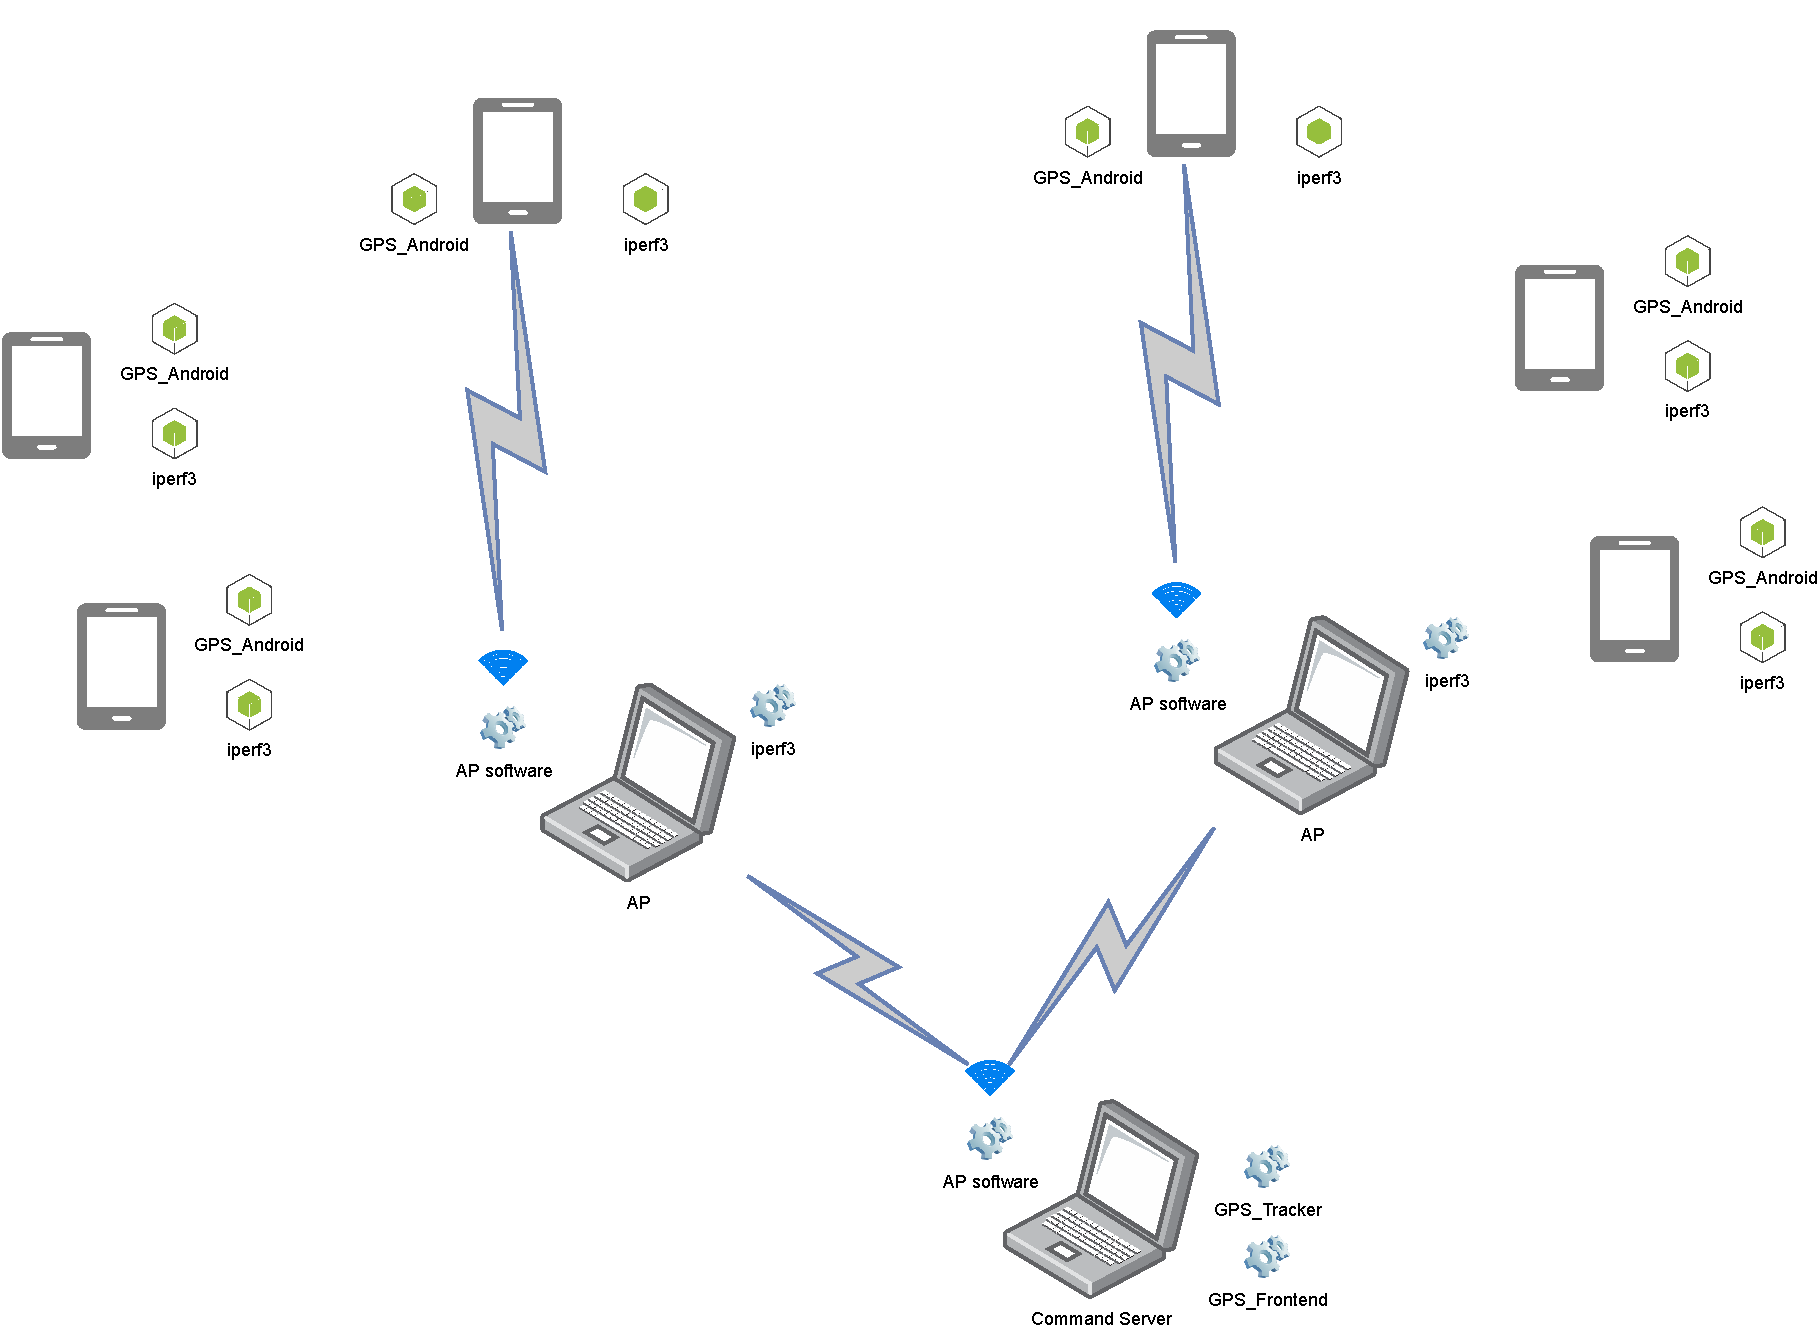
\includegraphics[width=\linewidth,keepaspectratio]{images/Deployment Diagram-Free-structure_scheme.pdf}
\caption{Main scenario of the experiment}
\label{fig:experiment-overall-layout}
\end{figure}

From the general system engineering perspective, the experiment is a set
of wireless-connected nodes (via Wi-Fi 802.11n (300 mbps)) which measures the receiving signal strength and measure the throughput of the link to upload and download.

All connections are wireless on each bearer:

\begin{itemize}
\tightlist
\item
  UE \textless{}-\textgreater{} AP.
\item
  AP \textless{}-\textgreater{} CnC.
\end{itemize}

There investigated one problem: the experimental network bandwidth
between UE and AP measurements with \texttt{iperf3} showed about
\textbf{30 MBit/s} speed rate. On the contrary, speed on the bearer UE \textless{}- AP -CnC\textgreater{} showed about \textbf{12-15 MBit/s} speed rate. There is markedly seen a drop in speed rate, probably, because of transmission on the radio channel two-times. The problem  is not in the Wi-Fi itself, but in the fact that radio (wireless) link is not as reliable, as a cord one, so the active bandwidth measurement part must be located as close to the APs as possible - in our case, the server-side \texttt{iperf3} is located in \gls{access_point}.

Each UE has two programs on board:

\begin{itemize}
\tightlist
\item
  \texttt{GPS\_Android} - special software designed to perform \acrshort{rss} and  link measurements linked to GPS coordinates.
\item
  \texttt{Magic\ iperf} - a network bandwidth measurement software.  Provides a user-friendly interface to client-side app \texttt{iperf}  on Android phones.
\end{itemize}

Each APs has two Wi-Fi adapters. Since we use laptops to run APs, they expected to have one already included, thus one external extra required for each AP. The internal Wi-Fi adapter connects to the CnC provided Wi-Fi network, the external Wi-Fi adapter creates the access point named
``\textbf{ap}'' for the UEs.

The CnC uses one external AP to create the access point named
``\textbf{cnc}''.

\subsection{Deployment Diagram}\label{deployment-diagram}

\begin{longtable}[]{@{}ll@{}}
\caption{The main deployed components.}\tabularnewline
\toprule
\begin{minipage}[b]{0.16\columnwidth}\raggedright
Component\strut
\end{minipage} & \begin{minipage}[b]{0.78\columnwidth}\raggedright
Description\strut
\end{minipage}\tabularnewline
\midrule
\endfirsthead
\toprule
\begin{minipage}[b]{0.16\columnwidth}\raggedright
Component\strut
\end{minipage} & \begin{minipage}[b]{0.78\columnwidth}\raggedright
Description\strut
\end{minipage}\tabularnewline
\midrule
\endhead
\begin{minipage}[t]{0.16\columnwidth}\raggedright
Android smartphone group (UEs)\strut
\end{minipage} & \begin{minipage}[t]{0.78\columnwidth}\raggedright
A set of smartphones running Android OS (version 5.0+) with dedicated
Wi-Fi and installed software.\strut
\end{minipage}\tabularnewline
\begin{minipage}[t]{0.16\columnwidth}\raggedright
Access points (APs)\strut
\end{minipage} & \begin{minipage}[t]{0.78\columnwidth}\raggedright
The computers running a Wi-Fi AP software for the UEs connection. Pass
traffic through to CnC and take part in RSS and link quality
measurement.\strut
\end{minipage}\tabularnewline
\begin{minipage}[t]{0.16\columnwidth}\raggedright
Command Center (CnC)\strut
\end{minipage} & \begin{minipage}[t]{0.78\columnwidth}\raggedright
A computing node running the optimization software. Should be provided
with sufficient hardware resources.\strut
\end{minipage}\tabularnewline
\bottomrule
\end{longtable}

From the deployment view, we are using a complicated combination of
software and hardware.

We prefer to run AP and designed software separately in a virtual
machine. That helps to automate development, testing, and maintenance
routines.

\begin{figure}[H]
\centering
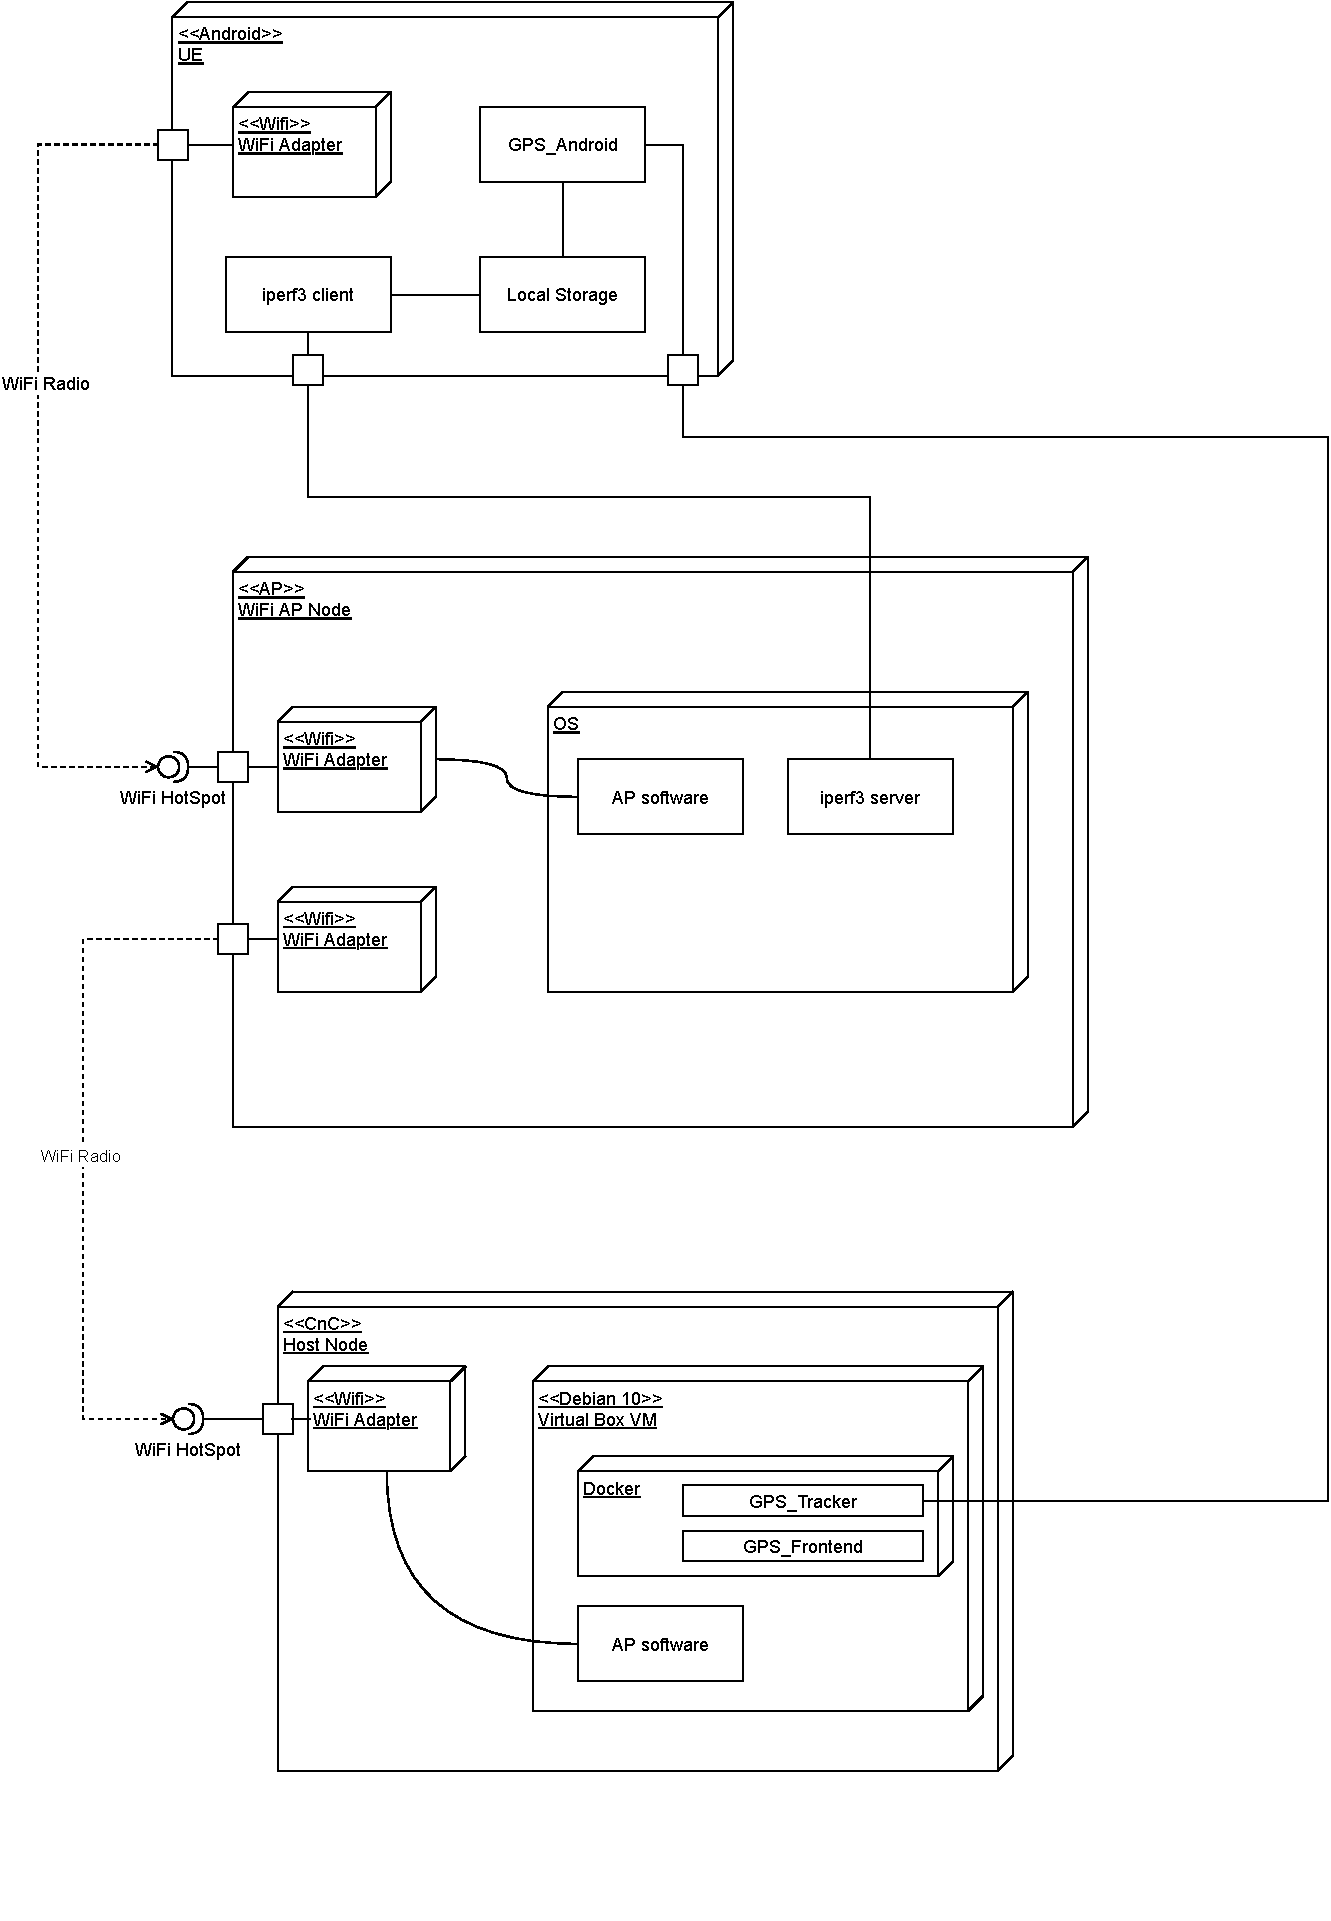
\includegraphics[width=\linewidth, keepaspectratio]{images/Deployment Diagram-Deployment_Diagram.pdf}
\caption{Deployment Diagram}
\label{fig:deployment-diagram}
\end{figure}

\subsubsection{Command center deployment
(CnC)}\label{command-center-deployment-cnc}

The CnC software runs on Debian OS in VirtualBox virtual machine.
\texttt{GPS\_Tracker} and \texttt{GPS\_Frontend} are designed to run in
Docker containers. For the experiment, the virtual machine has \textbf{docker}
and \textbf{docker-compose} installed to run these containers. It possible to have performance decrease because of running in containers, however more powerful hardware resources compensates those possible consequences of additional run-time level.

The AP software consists of two packages:

\begin{itemize}
\tightlist
\item
  \texttt{hostapd} - software to manage and run Wi-Fi access points.
\item
  \texttt{dnsmasq} - DNS/DHCP server, to provide an IP address, routing
  and DNS information via DHCP protocol.
\end{itemize}

The AP software starts in the virtual machine, which can access the physical Wi-Fi adapter using the hardware pass-through function from the host machine.

For easy-to-run configuration and deployment of the CnC, there are
provided an \textbf{Ansible} script.

\subsubsection{Access Points deployment
(APs)}\label{access-points-deployment-aps}

Unlike CnC, physical nodes run the AP software and server-side
\texttt{iperf3} app.

\subsection{Network Diagram}\label{network-diagram}

The APs subnet has identical settings. These
\texttt{Wi-Fi\ HotSpot\ Network} has an internal DHCP server to provide
dynamic addresses for connected UEs. To prevent the network IP addresses
collisions and simplify routing, the APs perform masquerading
(SNAT/DNAT) on the output interface (the internal interface used to
connect to CnC). On the one side, it cannot access the UEs directly from
CnC, but the UEs will always reach CnC as long as DHCP sets the default
gateway IP address.

In \texttt{Wi-Fi\ CnC\ Network} installed another DHCP server. It used
to reply to connecting APs with dynamic addresses. Because the subnet
used in this network is different from the internal Wi-Fi adapter's
network in the APs, there is no network collision.

Finally, the UEs can access the static CnC address \texttt{192.168.20.1}
as well as its local AP's gateway address \texttt{192.168.10.1}.


\begin{figure}[H]
	\centering
	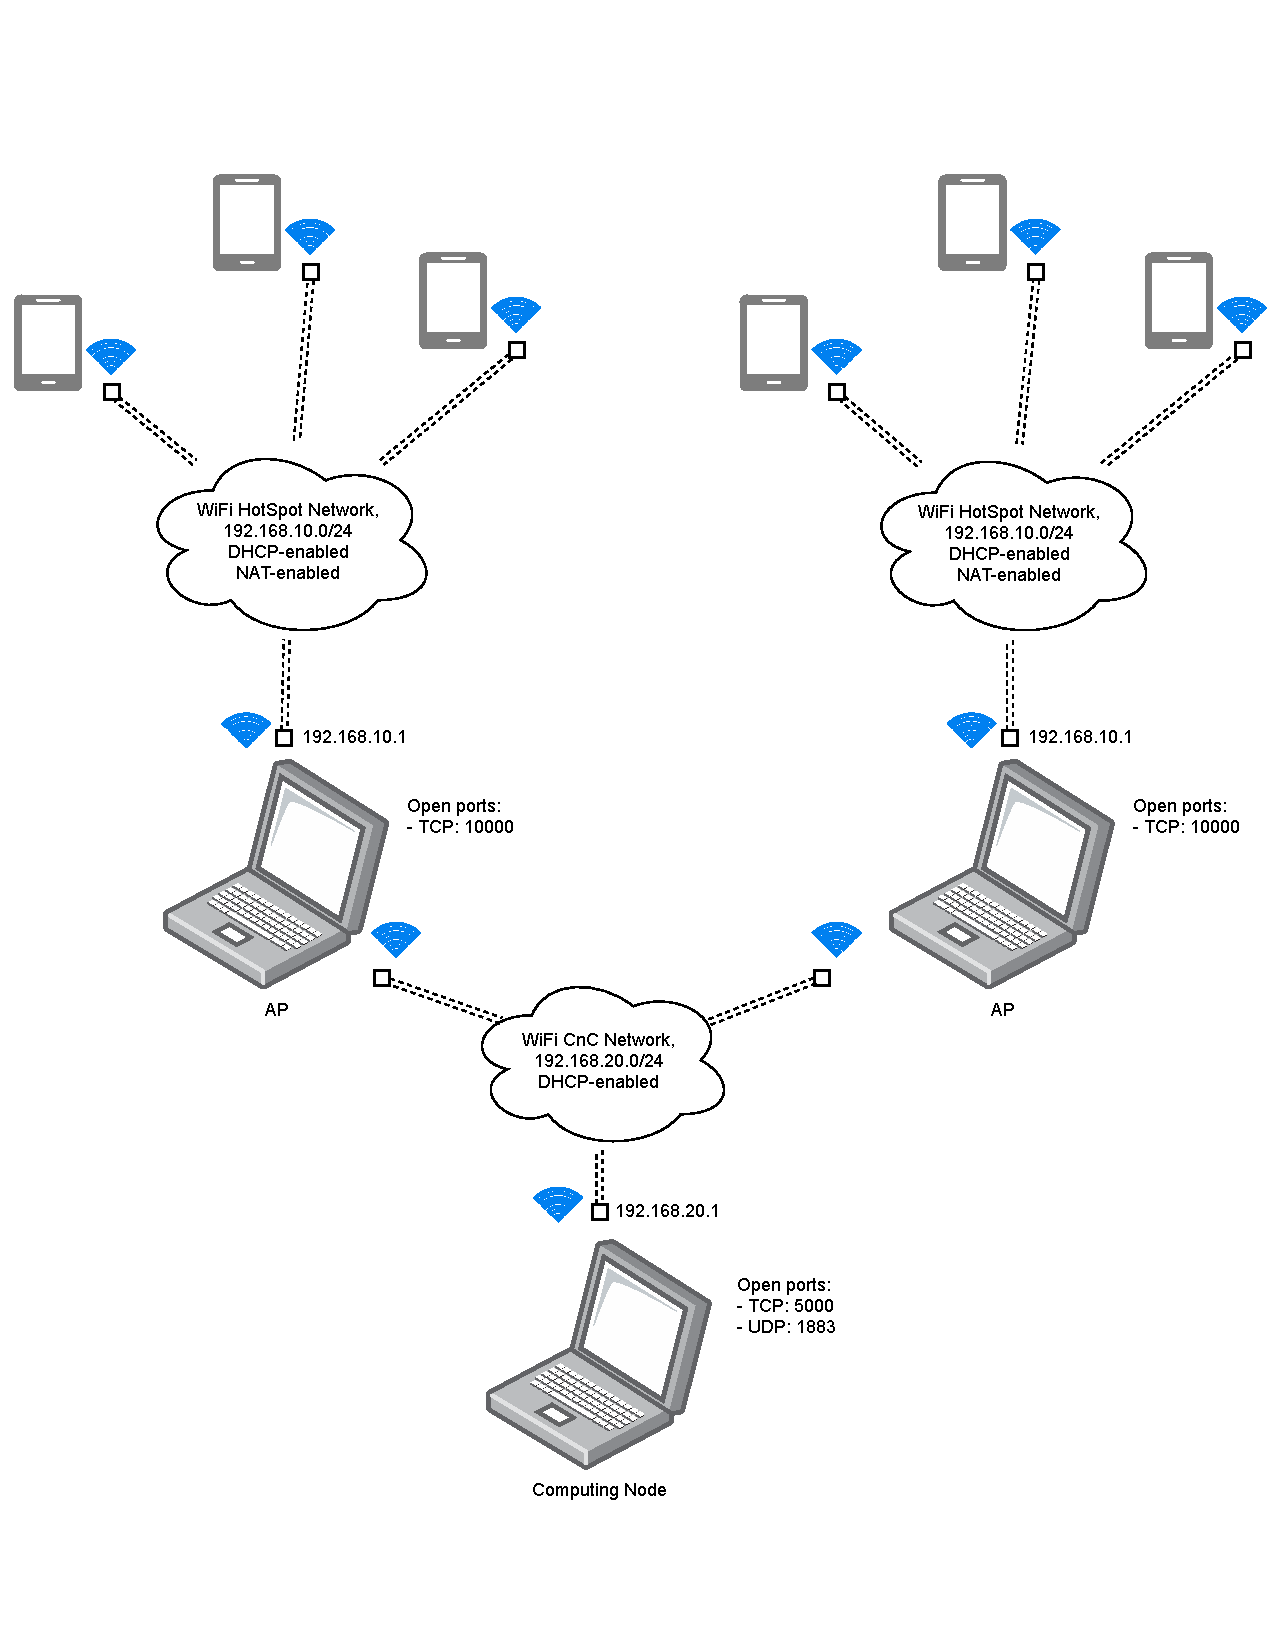
\includegraphics[width=\linewidth, keepaspectratio]{images/Deployment Diagram-Network_Diagram.pdf}
\caption{Network Diagram}
\label{fig:network-diagram}
\end{figure}

\subsection{Experiment Steps}\label{experiment-steps}

The following steps will be executed for each described experimental
case:

\begin{longtable}[]{@{}lll@{}}
\caption{Steps for one experimental case.}\tabularnewline
\toprule
\begin{minipage}[b]{0.01\columnwidth}\raggedright
No\strut
\end{minipage} & \begin{minipage}[b]{0.35\columnwidth}\raggedright
Step\strut
\end{minipage} & \begin{minipage}[b]{0.55\columnwidth}\raggedright
Description\strut
\end{minipage}\tabularnewline
\midrule
\endfirsthead
\toprule
\begin{minipage}[b]{0.01\columnwidth}\raggedright
No\strut
\end{minipage} & \begin{minipage}[b]{0.35\columnwidth}\raggedright
Step\strut
\end{minipage} & \begin{minipage}[b]{0.55\columnwidth}\raggedright
Description\strut
\end{minipage}\tabularnewline
\midrule
\endhead
\begin{minipage}[t]{0.01\columnwidth}\raggedright
1\strut
\end{minipage} & \begin{minipage}[t]{0.35\columnwidth}\raggedright
Initialize network connectivity between APs and CnCs\strut
\end{minipage} & \begin{minipage}[t]{0.55\columnwidth}\raggedright
Ensure that these nodes are available in the network by the ICMP
protocol\strut
\end{minipage}\tabularnewline
\begin{minipage}[t]{0.01\columnwidth}\raggedright
2\strut
\end{minipage} & \begin{minipage}[t]{0.35\columnwidth}\raggedright
Run the software for the experiment\strut
\end{minipage} & \begin{minipage}[t]{0.55\columnwidth}\raggedright
Startup GPS\_Tracker, GPS\_Frontend\strut
\end{minipage}\tabularnewline
\begin{minipage}[t]{0.01\columnwidth}\raggedright
3\strut
\end{minipage} & \begin{minipage}[t]{0.35\columnwidth}\raggedright
Place the APs and UEs according to an experiment case\strut
\end{minipage} & \begin{minipage}[t]{0.55\columnwidth}\raggedright
There are specific predefined positions for each element on the
experiment area.\strut
\end{minipage}\tabularnewline
\begin{minipage}[t]{0.01\columnwidth}\raggedright
4\strut
\end{minipage} & \begin{minipage}[t]{0.35\columnwidth}\raggedright
Measure RSS, Link quality for the initial layout\strut
\end{minipage} & \begin{minipage}[t]{0.55\columnwidth}\raggedright
Measurements are done via GPS\_Android that sends the result to
GPS\_Tracker\strut
\end{minipage}\tabularnewline
\begin{minipage}[t]{0.01\columnwidth}\raggedright
5\strut
\end{minipage} & \begin{minipage}[t]{0.35\columnwidth}\raggedright
Run the APs location optimization for each algorithm in
GPS\_Tracker\strut
\end{minipage} & \begin{minipage}[t]{0.55\columnwidth}\raggedright
Each optimization algorithm can produce different probable positions for
the same UE positions and measurements.\strut
\end{minipage}\tabularnewline
\begin{minipage}[t]{0.01\columnwidth}\raggedright
6\strut
\end{minipage} & \begin{minipage}[t]{0.35\columnwidth}\raggedright
Move the APs to the optimized positions\strut
\end{minipage} & \begin{minipage}[t]{0.55\columnwidth}\raggedright
It is expected that new positions for APs would increase our network
efficiency.\strut
\end{minipage}\tabularnewline
\begin{minipage}[t]{0.01\columnwidth}\raggedright
7\strut
\end{minipage} & \begin{minipage}[t]{0.35\columnwidth}\raggedright
Repeat RSS and Link quality measurements for the optimized APs
positions\strut
\end{minipage} & \begin{minipage}[t]{0.55\columnwidth}\raggedright
1-3 interactions for optimization per each case.\strut
\end{minipage}\tabularnewline
\bottomrule
\end{longtable}

	\hypertarget{case-1.-sub-optimal-layout}{%
\section{Case-1. Sub-optimal layout}\label{case-1.-sub-optimal-layout}}

In the first case \textbf{Access Points(APs)} are placed in the ground
so that both of them are in the center of the corresponding quarter of
25x25 meters and far from all UEs to approximately 25 meters.

\textbf{UEs} are left in two groups of three filling the other two
quarters respectively.

At the same time, they are not too close to each other in order to not
have interference and absolutely the same conditions.

Finally, \textbf{CnC} is set in the middle of the whole 50x50 meters an
experimental field, so that 2 APs and 2 groups of UEs mentioned above
are on the same distance.

This case expects to perform in the best signal quality and transmission
rate.

\begin{figure}[H]
	\centering
	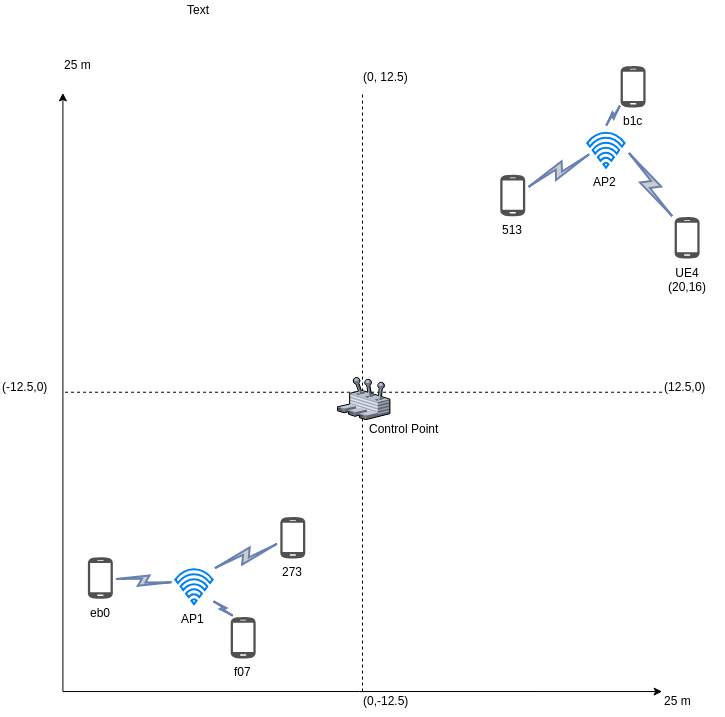
\includegraphics[width=\linewidth,keepaspectratio]{images/05-cases-description-Exp4-Suboptimal.png}
\caption{Near-optimal layout example}
\end{figure}

	\section{Uniform layout}\label{uniform-layout}

In the uniform case layout, presented in Figure \ref{fig:uniform-case-layout}, we want to put \glspl{ap} at the same distance and line from \gls{command_n_center}.

Here, both \glspl{ap} are set right on the line between the 1st and 3rd quarters and between the 2nd and 4th quarters.

Signal quality and transmission rate in this configuration expected to increase compared with the \hyperref[near-optimal-layout]{Near-Optimal case}.

\begin{figure}[H]
	\centering
	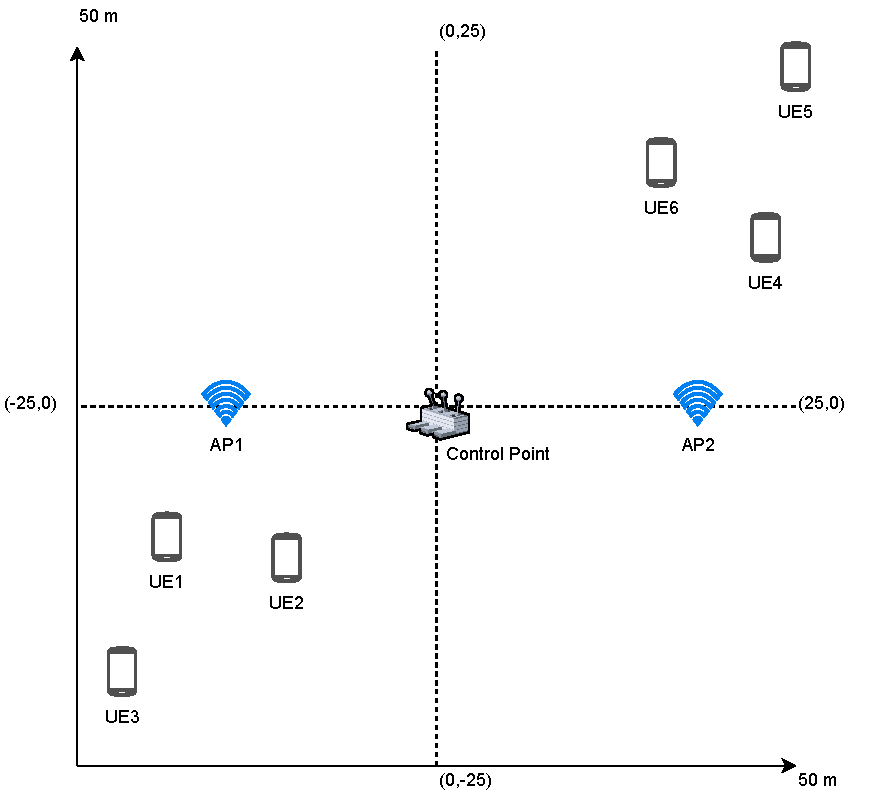
\includegraphics[width=0.7\linewidth,keepaspectratio]{images/05-cases-description-Uniform.pdf}
	\caption{Uniform case layout}
	\label{fig:uniform-case-layout}
\end{figure}

	\section{Case-3. Sub-optimal layout}\label{case-3.-near-optimal-layout}

In the third case, the only changed things are the position of
\textbf{APs}.

Each of them now is put in the middle of each group of 3 UEs, therefore
they have the same distance to centers of each cluster.

This case expects to perform in the best signal quality and transmission rate.

\begin{figure}[H]
	\centering
	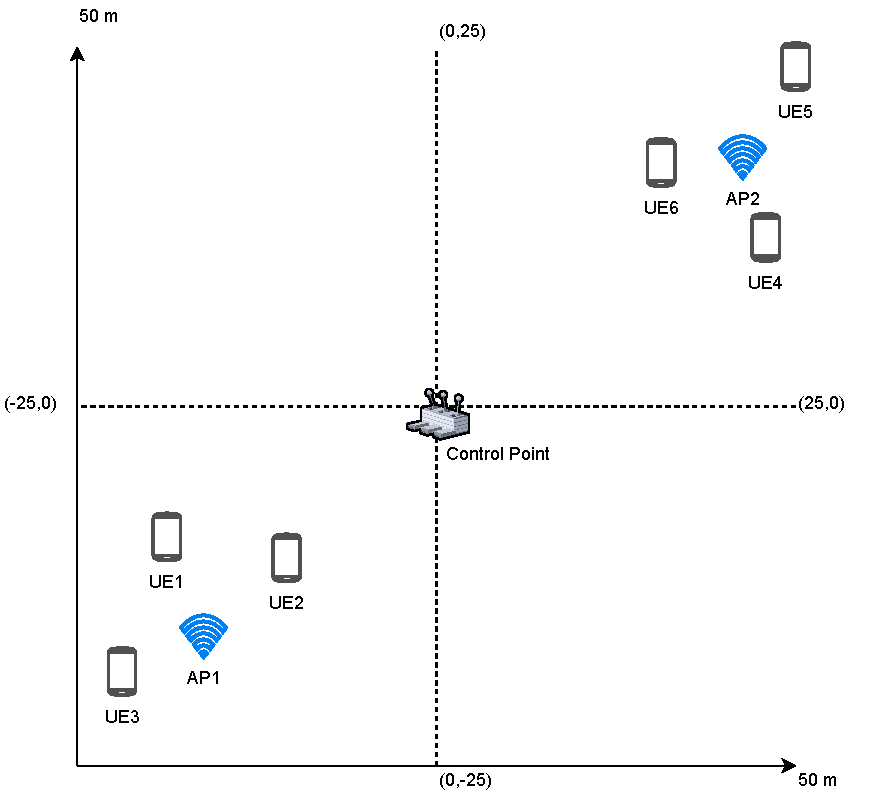
\includegraphics[width=\linewidth,keepaspectratio]{images/05-cases-description-Sub-optimal.pdf}
\caption{Near-optimal layout example}
\end{figure}

	\section{Experimental Phase}\label{experimental-phase}

	\hypertarget{experiment-1.-12.02.2020}{%
\subsection{Experiment-1. 12.02.2020}\label{experiment-1.-12.02.2020}}

The first attempt took place on 12.02.2020.

The aim was to involve as many UEs as possible. This is the reason for performing the experiment on that day. Eventually, \textbf{6 UEs} took part ranging by the Android version from 4 to 9.

Besides, the installation of apps and binding Wi-Fi to the necessary
access point, a detailed \textbf{journal of the Wi-Fi} connection
information enabled. This allowed monitoring RSS value on each UE.

\hypertarget{weather-conditions}{%
\subsection{Weather conditions}\label{weather-conditions}}

\begin{itemize}
\tightlist
\item
  no precipitation
\item
  cloudy sky
\item
  a thin layer of snow on the ground
\item
  temperature of -1..+1
\end{itemize}

\hypertarget{procedure}{%
\subsection{Procedure}\label{procedure}}

All items of the experiment placed on the carton boxes on the ground, so that they are a bit raised from the ground.

\begin{figure}[H]
	\centering
	\includegraphics[width=\linewidth,keepaspectratio]{images/experiment_1_cnc.jpg}
\caption{Layout of CnC server}
\end{figure}

\hypertarget{case-1}{%
\subsubsection{Case 1}\label{case-1}}

\textbf{Suboptimal scheme} was chosen to begin with: UEs' connection to one AP was made successfully.

The second AP was connected to the other 3 UEs with more effort. The reason for it was in the Wi-Fi module issues of AP  (the laptop freeze).

After some time of data collection, it was clear the second AP was not sending data to CnC at all, so we decided to locate devices according to the near-optimal scheme.

\hypertarget{case-2}{%
\subsubsection{Case 2}\label{case-2}}

This helped to increase the RSS level a bit from -82 and -84 to -76 and
-80, data still was collected only from the first AP.

Besides, the graphical view in CnC showed 4 UEs close to each other (having approximately the same GPS coordinate), whereas the other 2 were detected much further.

Then we figured out that the second AP stopped working at some time. Restart and re-connection of UEs did not help to obtain data of that 3 UEs in CnC.

\hypertarget{case-3}{%
\subsubsection{Case 3}\label{case-3}}

It made no sense to try without data collection on CnC.

\hypertarget{outcome}{%
\subsection{Outcome}\label{outcome}}

The first attempt of the experiment showed:

\begin{itemize}
\tightlist
\item
  Further development of GPS\_Tracker and GPS\_Android to fix bugs required.
\item
  Tests of placement algorithms performing, but due to problem with message communication, we were unable to test if the optimized positions would lead to better signal conditions.
\end{itemize}

As a result, we decided to:

\begin{itemize}
\tightlist
\item
  fix the second AP failure reasons
\item
  figure out the source of 2 point-outliers in the plot
\end{itemize}

	\hypertarget{experiment-1.-22.02.2020}{%
\subsection{Experiment-1. 22.02.2020}\label{experiment-1.-22.02.2020}}

The second attempt took place on 22.02.2020.

This time the aim was to check how \textbf{updates} in different parts
of the system behave in real condition:

\begin{itemize}
\tightlist
\item
  a new way to estimate load speed in-app
\item
  possibility to read app logs right on UE
\item
  improved front-end part
\end{itemize}

The goal did not include a full-scale experiment with as many devices
involved, so there were 1 CnC, 1 AP, and 3 UEs with the same settings
from the previous experiment but updated app.

\hypertarget{weather-conditions}{%
\subsection{Weather conditions}\label{weather-conditions}}

\begin{itemize}
\tightlist
\item
  no precipitation
\item
  clear sky
\item
  no snow
\item
  strong winds
\end{itemize}

\hypertarget{procedure}{%
\subsection{Procedure}\label{procedure}}

Only one case (near-optimal) was performed.

\begin{figure}[H]
	\centering
	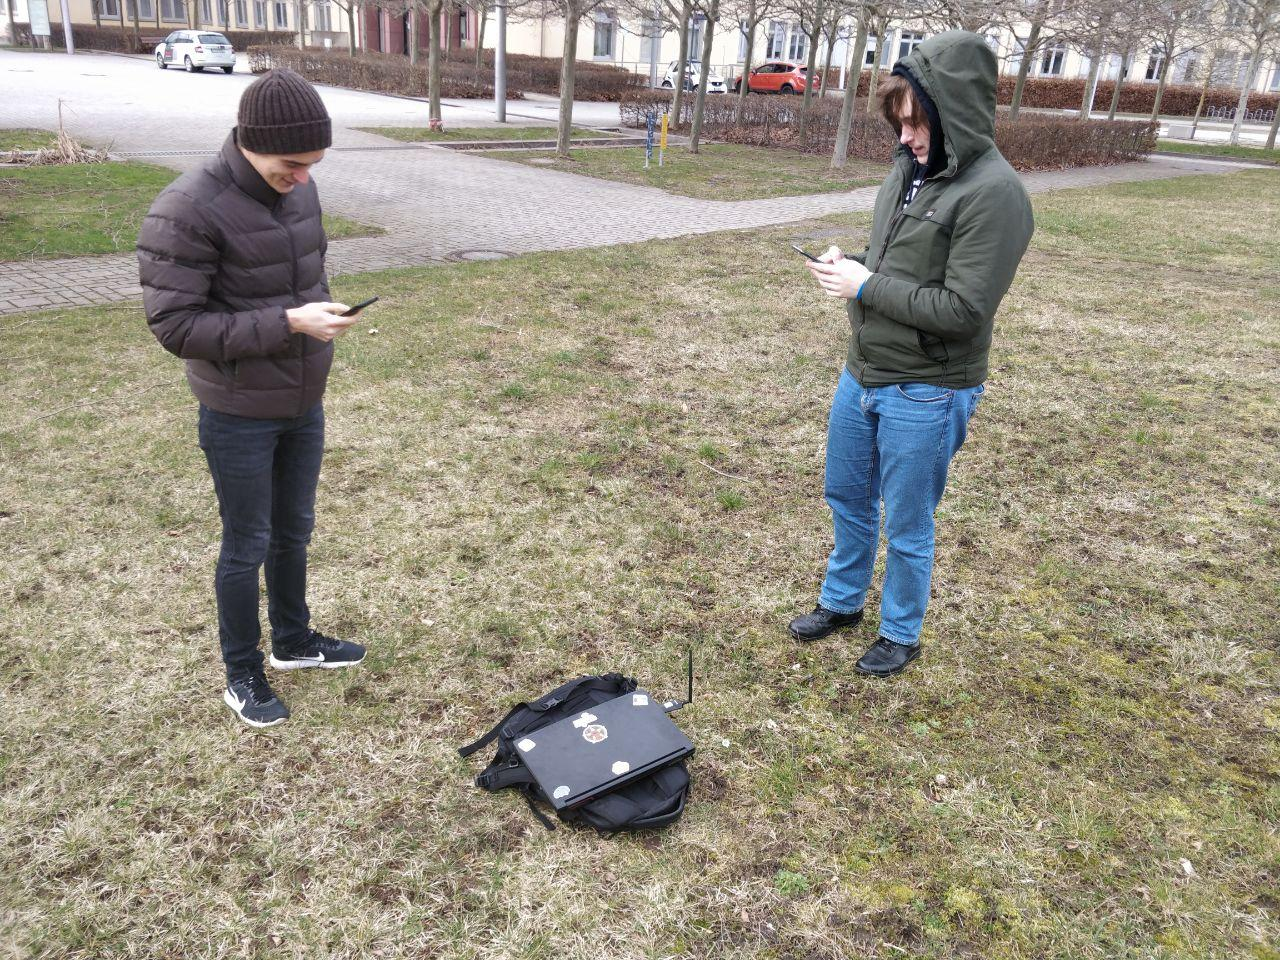
\includegraphics[width=\linewidth,keepaspectratio]{images/experiment_2_overview.jpg}
\caption{The initial CnC server position}
\end{figure}

All the UEs connections made successfully:

\begin{itemize}
\tightlist
\item
  deviceId assigned
\item
  UE coordinates displayed
\end{itemize}

During the first half of the experiment time, after pressing `push once'
\textbf{upload/download speeds} were estimated and displayed, although
the values seemed to be not realistic (300 000 kBit/s). The values were
much smaller when CnC was not connected to the Internet.

Later, pressing `push once' did not cause speed re-estimation, and logs
contained error messages about issues related to the MQTT.

\hypertarget{outcome}{%
\subsection{Outcome}\label{outcome}}

The second attempt was also not successful. We hadn't managed to solve
the problem in telemetry data sending, some design proposals can be a
solution for the next iteration.

As a result, we decided to:

\begin{itemize}
\tightlist
\item
  add logging to APs as well
\item
  implement direct HTTP requests
\end{itemize}

	\section{Experiment 3. 07.02.2020}\label{experiment-3.-07.02.2020}

It took place on 27.02.2020. We aimed to check how \textbf{2 major updates} of the \gls{android} app behave.

The \emph{first} update concerns the usage of \gls{http} requests instead of \gls{mqtt}. We suspected that \gls{mqtt}-protocol is the reason of previously detected issues.

The \emph{second} update is to refactor the source code. It includes switching to \gls{mvvm} architectural pattern, removing of insignificant interface components.

\subsection{Procedure}

Due to the bad weather conditions (heavy snowfall), we decided to perform experiments indoor (Mensa). Mensa is a 2-floor building in TU Ilmenau, it has a large area inside.

The layout included 1 \gls{command_n_center}, 1 \gls{ap}, and 3 \glspl{ue} took part.

All \glspl{ue} can connect to \gls{command_n_center} successfully:

\begin{itemize}
	\tightlist
	\item
	`Push once' button pressed
	\item
	deviceId assigned
	\item
	UE coordinates displayed
\end{itemize}

\subsection{Consideration during the experiment}

As for `Push continuously', it should be known in advance the
coordinates updated on the display \textbf{only in the case of moving to some minimal delta} (10 centimeters). This is insured based on \gls{gnss} values passed by the \gls{android} device.

To make sure the connection is still alive and the values are transferred, we checked the log journal periodically.

\subsection{Outcome}

To sum up, the system finally started working without failures and the meaningful set of data is collected, as shown in the following figures.



\begin{figure}[H]
	\centering
	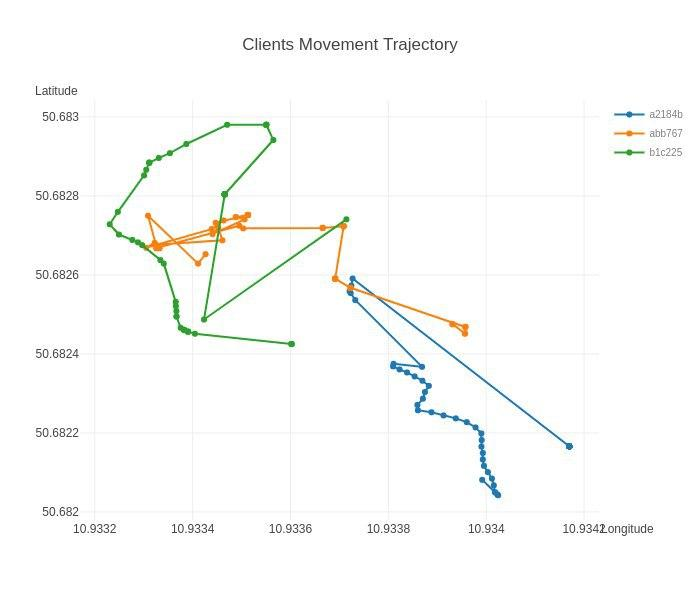
\includegraphics[width=0.5\linewidth,keepaspectratio]{images/experiment_3_1.jpg}
	\caption{Movement trajectory of connected phones}
	\label{fig:movement-trajectory}
\end{figure}

Figure \ref{fig:movement-trajectory} shows movement trajectory of connected clients. 

\begin{figure}[H]
	\centering
	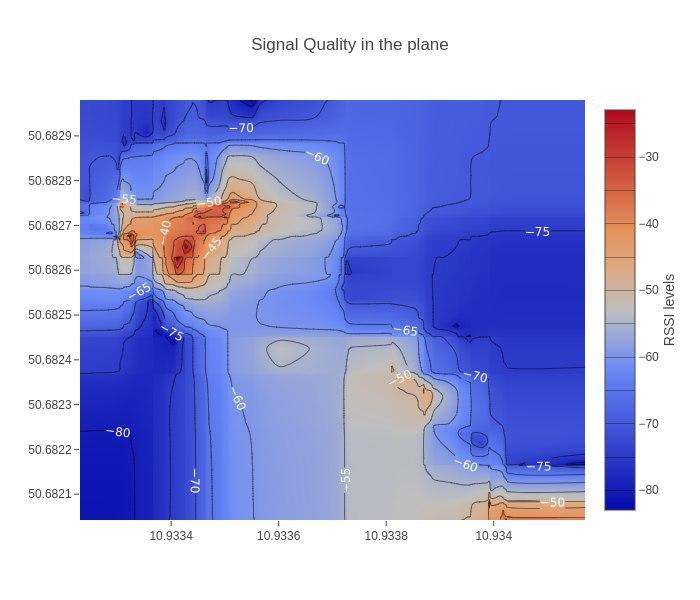
\includegraphics[width=0.5\linewidth,keepaspectratio]{images/experiment_3_2.jpg}
	\caption{Signal quality map}
	\label{fig:signal-quality-heatmap}
\end{figure}

Figure \ref{fig:signal-quality-heatmap} shows how signal changes in different location inside Mensa. Due to obstacles (concrete walls, metal objects), the signal rapidly decreases in the farthest corners and on the second floor.

Figure \ref{fig:signal-quality-changes} describes changes in \acrshort{rss} while \glspl{ue} were moving inside the building. It is clear to observe that some phones started transmitting later than others. If a \gls{ue} fails to send a measurement message, it stores in a local database and resends once the connection is back.


\begin{figure}[H]
	\centering
	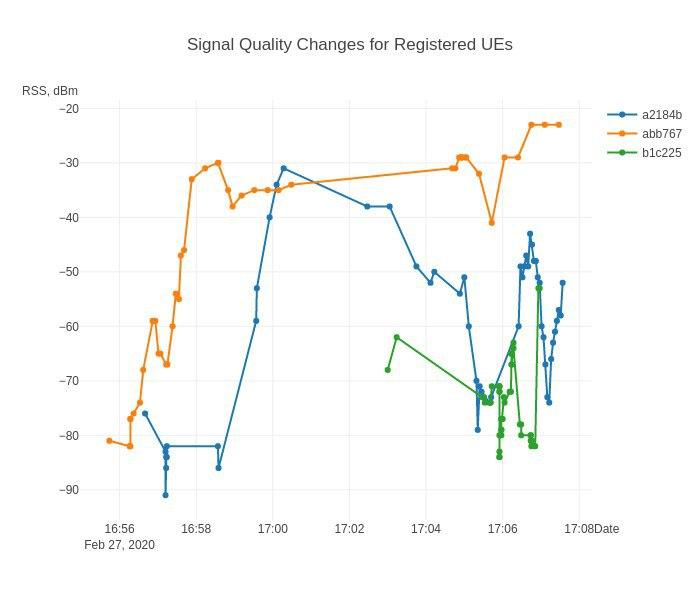
\includegraphics[width=0.5\linewidth,keepaspectratio]{images/experiment_3_3.jpg}
	\caption{Signal quality changes}
	\label{fig:signal-quality-changes}
\end{figure}

	\section{Experiment 4. 03.03.2020}\label{experiment-4.-03.03.2020}

It took place on 03.03.2020. The weather condition was appropriate for running experiments, despite that it was raining lightly.

For the fourth attempt, we implement message sending only via HTTP. The main aim of the experiment is to find optimized positions for the UEs in three cases (sub-optimal, uniform, near-optimal). Phones forced to push their channel quality metric to the server for each case. On the server-side, GPS\_Tracker tries to find optimal positions for UAVs supposing there are 2 AP is required.

We decided to reduce the area layout to 25x25 meters.

\subsection{Results}

The HTTP protocol helps us to receive messages more reliable, although there was a problem, e.g. the further UE is located from AP, the less is probable the reception of the message.

Tests showed reliability of HTTP protocol, therefore, we decided to continue our experiment.

We found out that network speed measurements were not significant, because there was markedly seen difference between uplink and downlink speed, uplink tests threw the timeout exception in case of larger distance between a UE and used AP, since the communication took longer and the session finished.

The measurements showed the following coordinates for the 6 UEs:

\begin{longtable}[]{@{}ll@{}}
\caption{Initial positions for UEs}\tabularnewline
\toprule
Unique ID & Coordinates\tabularnewline
\midrule
\endfirsthead
\toprule
Unique ID & Coordinates\tabularnewline
\midrule
\endhead
f072f812f48ce468 & (50.4056203, 10.5626057)\tabularnewline
eb0b54819c69cf0c & (50.4056230, 10.5626126)\tabularnewline
27349a2cde6592df & (50.4056445, 10.5625865)\tabularnewline
51336504999bc1ca & (50.40567855, 10.5625238)\tabularnewline
b1c225280d0ed13f & (50.4056924, 10.5624943)\tabularnewline
\bottomrule
\end{longtable}

The experiment is divided into four parts:

\begin{itemize}
\tightlist
\item
  Before 11:05 - sub-optimal case
\item
  11:05 - 11:08 - uniform case
\item
  11:08 - 11:12 - near-optimal case
\item
  11:12 - 11:15 sub-optimal to compare to the suggested positions
\end{itemize}

\subsubsection{Sub-optimal case}

The first case is the most profitable from the signal quality point of
view. The APs are implicitly located at the same distance from the
connected UEs. The level of interference is low.

\begin{figure}[H]
	\centering
	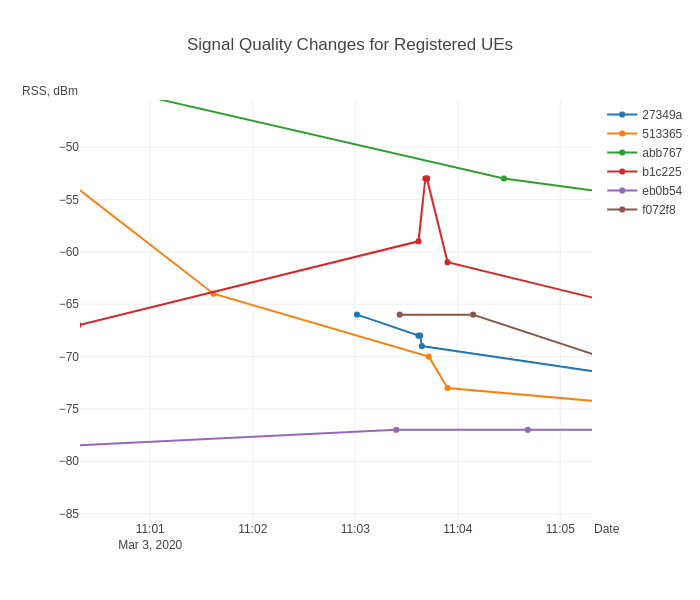
\includegraphics[width=\linewidth,keepaspectratio]{images/Exp4_Suboptimal.png}
\caption{Signal Quality changes in Sub-optimal case}
\end{figure}

Despite the APs were located close to UEs, the RSS level varies noticeably. However, only in this case the speed and signal quality measurement were the most stable among all cases.

\subsubsection{Uniform case}

In this case, the APs are located with equal distance from the CnC on the same line.

\begin{figure}[H]
	\centering
	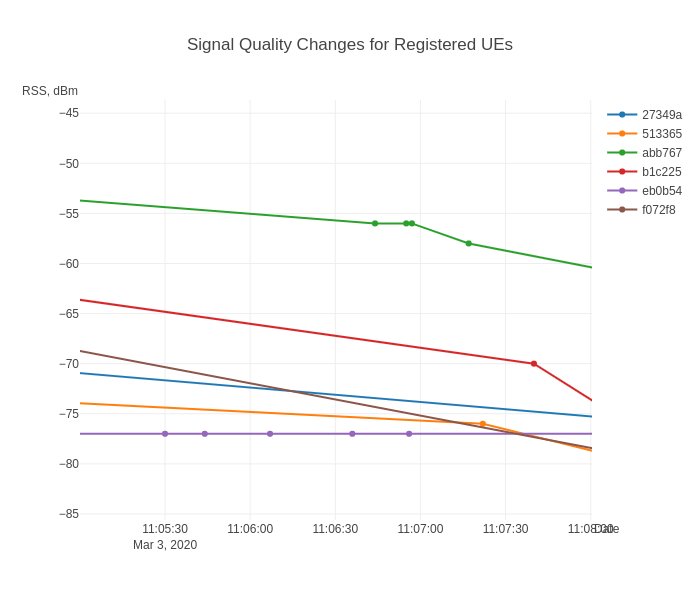
\includegraphics[width=\linewidth,keepaspectratio]{images/Exp4_Uniform.png}
\caption{Signal Quality changes in Uniform case}
\end{figure}

Link measurement became more smooth, but the speed test failed
sometimes.

\subsubsection{Near-optimal case}

The third case simulates the situation where the APs are placed
uniformly far from centers of UEs' clusters.

\begin{figure}[H]
	\centering
	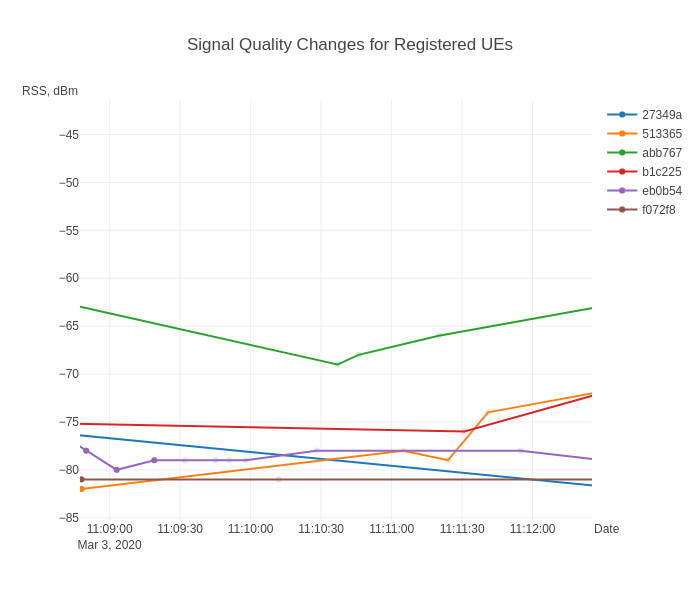
\includegraphics[width=\linewidth,keepaspectratio]{images/Exp4_Near_Optimal.png}
\caption{Signal Quality changes in Near-optimal case}
\end{figure}

\subsubsection{Comparison between Sub-optimal case, and the suggested
positions}

To check the validity of the UAVs layout optimization algorithm, we
place the APs in a Sub-optimal case position.

The given coordinates for \textbf{APs}:

\begin{longtable}[]{@{}ll@{}}
\toprule
AP & Coordinates\tabularnewline
\midrule
\endhead
AP1 & (50.4056741, 10.5625129)\tabularnewline
AP2 & (50.4056339, 10.5625975)\tabularnewline
\bottomrule
\end{longtable}

\begin{figure}[H]
	\centering
	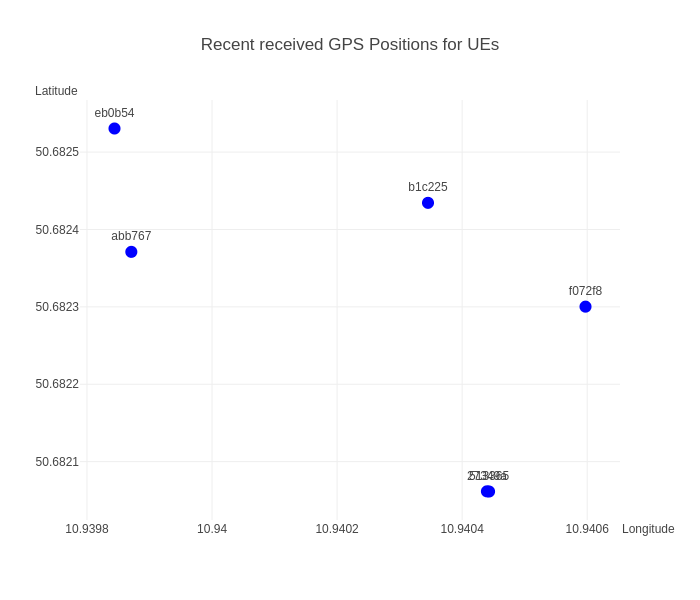
\includegraphics[width=\linewidth,keepaspectratio]{images/Exp4_UEs_Location_to_optimize.png}
\caption{The UEs coordinates used to optimize UAVs positions}
\end{figure}

The coordinates for \textbf{27349a2cde6592df} and
\textbf{51336504999bc1ca} overlap.

The most recent received coordinates for UEs used to schedule an
optimization task with the following parameters:

\begin{itemize}
\tightlist
\item
  Number of clusters: 2
\item
  Estimation method: ``clustering''
\end{itemize}

Using of ``simplex'' method against two clusters is not possible, produced result is unreliable.

\begin{figure}[H]
	\centering
	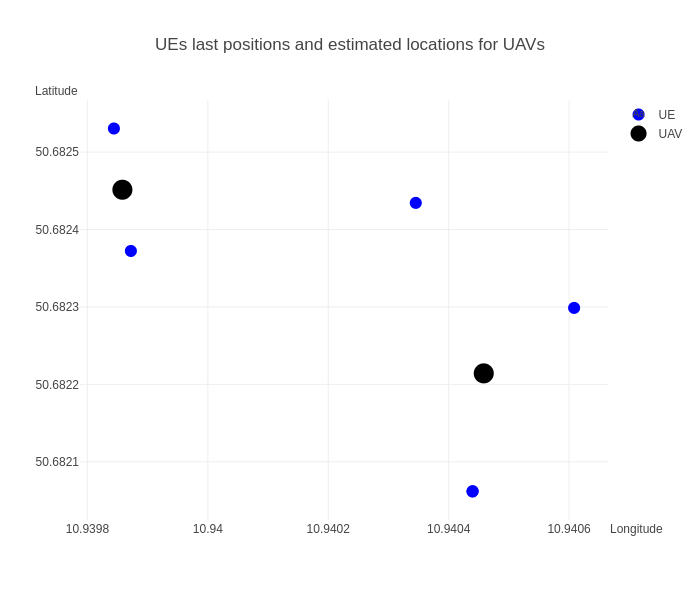
\includegraphics[width=\linewidth,keepaspectratio]{images/Expt4_Estimated UAVs_locations.png}
\caption{Black dots represent suggested points as the most optimal
position for UAVs}
\end{figure}

The suggested optimal coordinates for \textbf{APs}:

\begin{longtable}[]{@{}lll@{}}
\toprule
AP & Real coordinates & Optimal coordinates\tabularnewline
\midrule
\endhead
AP1 & (50.4056741, 10.5625129) & (50.68221, 10.94046)\tabularnewline
AP2 & (50.4056339, 10.5625975) & (50.68245, 10.93986)\tabularnewline
\bottomrule
\end{longtable}

\begin{figure}[H]
	\centering
	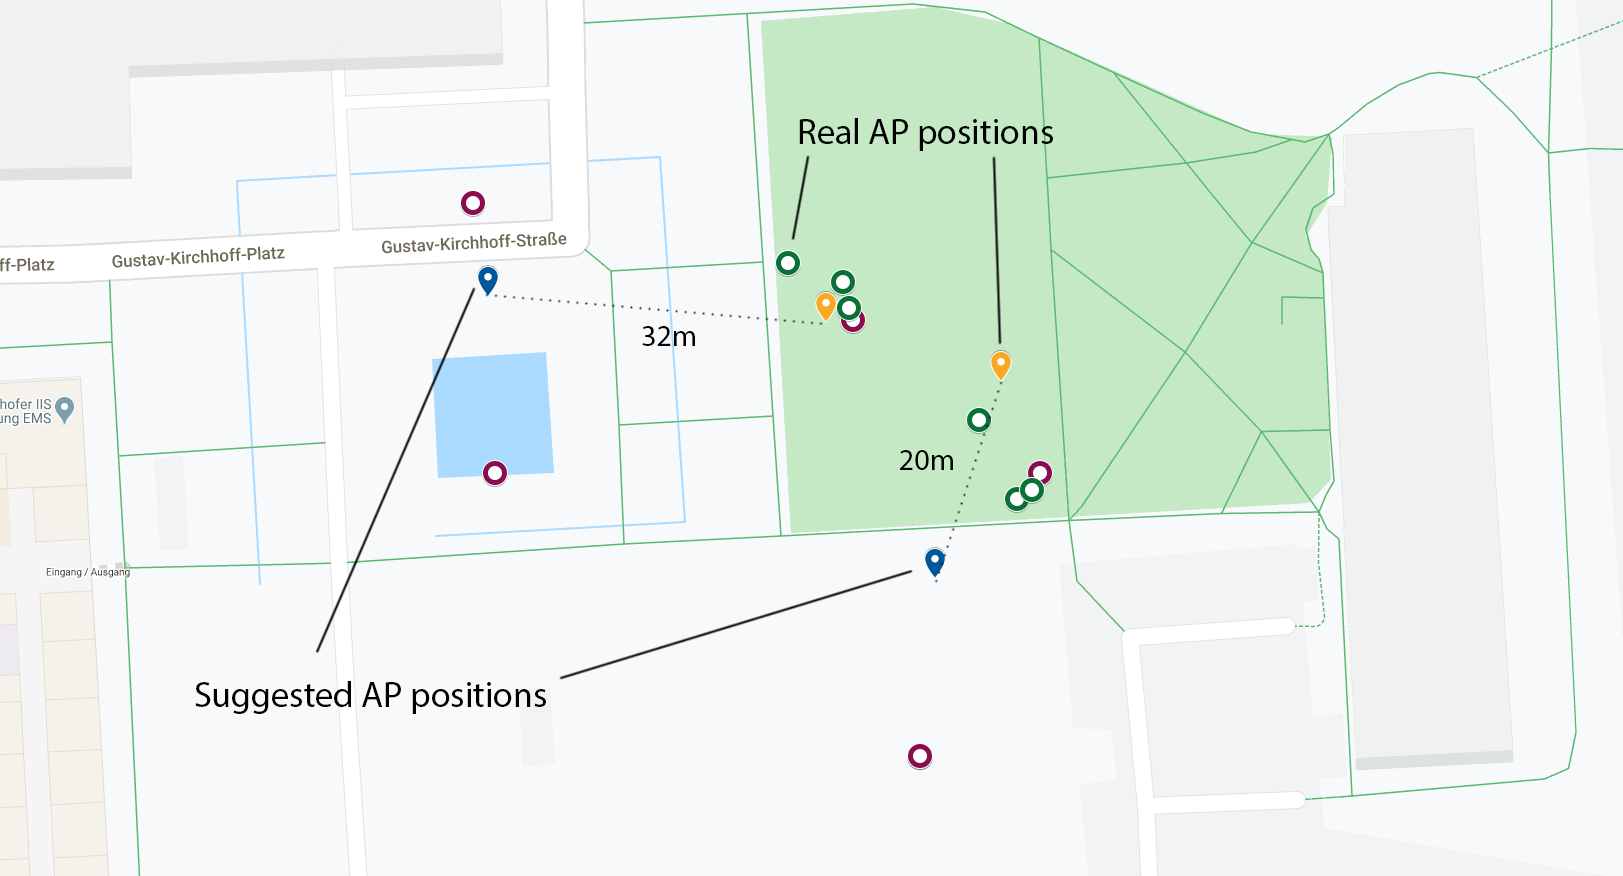
\includegraphics[width=\linewidth,keepaspectratio]{images/Expt4_Result_of_optimization_map_with_names.png}
\caption{Original and Optimized Coordinates: A map with tags. Clearly
seen the suggested ``optimal'' position can drop out connected clients
because of a large distance.}
\end{figure}

\begin{figure}[H]
	\centering
	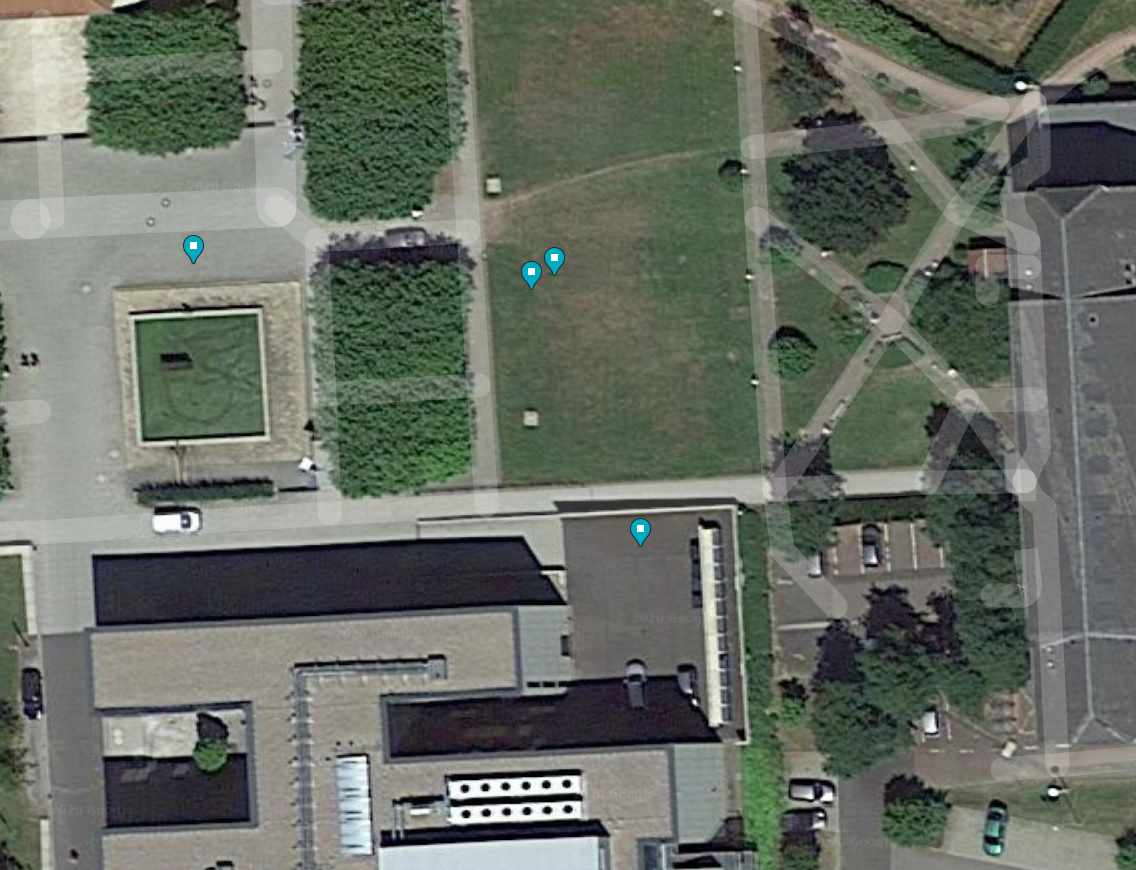
\includegraphics[width=\linewidth,keepaspectratio]{images/Expt4_Result_of_optimization_sattelite.png}
\caption{Original and Optimized Coordinates for UAvs: A picture from
satellite}
\end{figure}

``Clustering'' algorithm performs simple K-means cluster calculation
based on GPS coordinates for UEs. The result provides insights about
that layout optimization algorithms relying solely on the coordinate
input data can result in a biased solution.

\subsubsection{Pictures of experiment}

\begin{figure}[H]
	\centering
	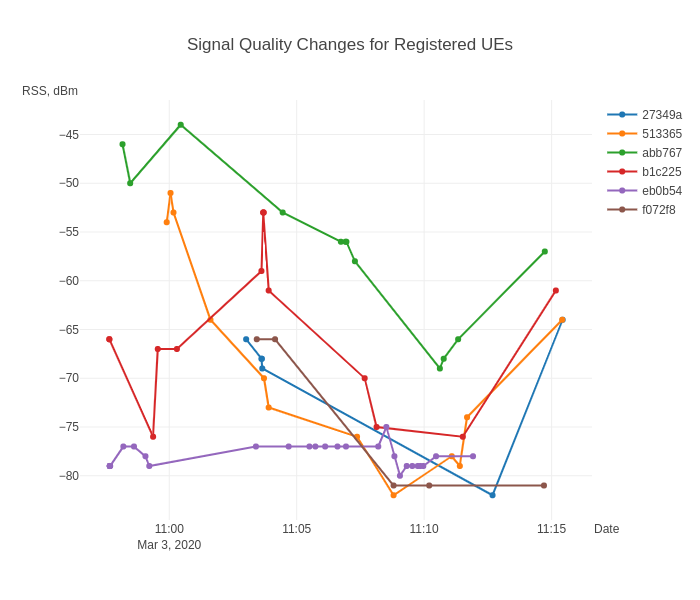
\includegraphics[width=\linewidth,keepaspectratio]{images/Exp4-Overall-Signal-Changes.png}
\caption{Signal Quality level changes during the experiment}
\end{figure}

\begin{figure}[H]
	\centering
	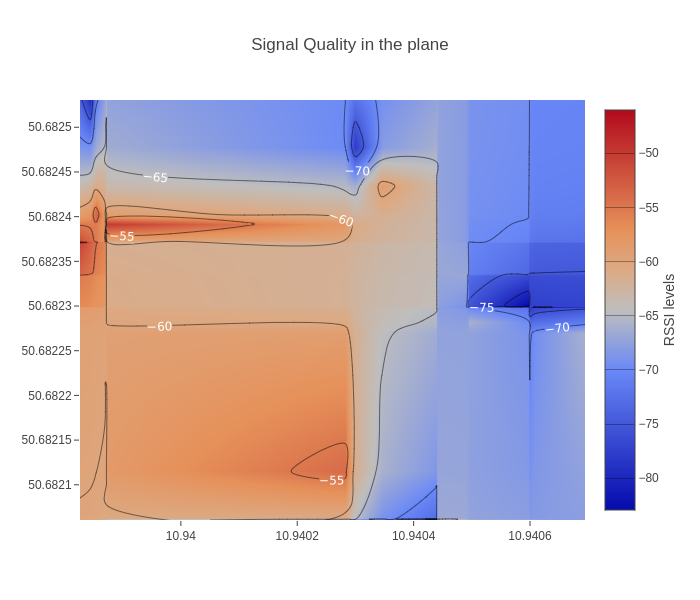
\includegraphics[width=\linewidth,keepaspectratio]{images/Exp4_Overall_Heatmap.png}
\caption{Signal Heatmap obtained during the experiment}
\end{figure}

\begin{figure}[H]
	\centering
	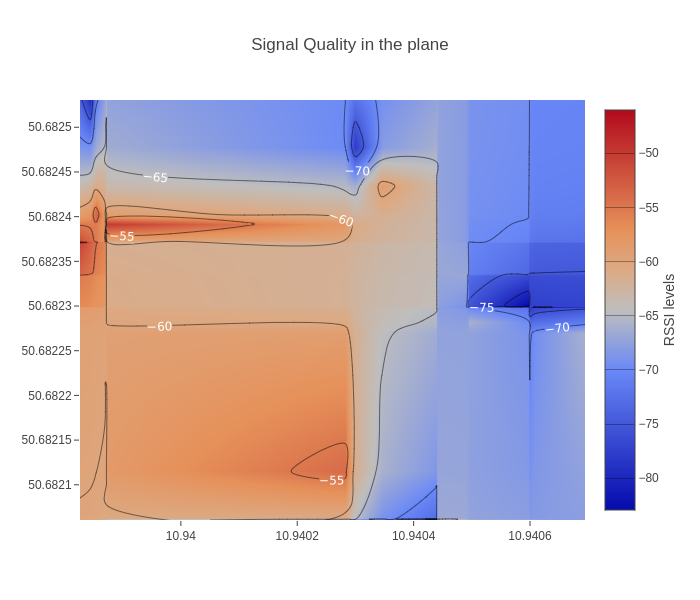
\includegraphics[width=\linewidth,keepaspectratio]{images/Exp4_Overall_Heatmap.png}
\caption{Signal Heatmap obtained during the experiment}
\end{figure}

\begin{figure}[H]
	\centering
	\includegraphics[width=\linewidth,keepaspectratio]{images/Layout_Problem_Discussion.jpg}
\caption{Layout Problem discussion}
\end{figure}

\subsection{Outcome}

Finally, we have managed to test the framework and estimate an optimized
position for UAVs which were represented by WiFi access points. The
results showed that the framework, as well as optimization algorithms,
should be redesigned and evaluated on updated data.

	\clearpage
\section{Final Results}\label{final-results}

We have completed 4 experimental attempts. We encountered problems each
attempt, mostly they cover:

\begin{itemize}
\tightlist
\item
  Wi-Fi connection: radio link may suffer serious collisions that drop
  up data transmission.
\item
  Complicated architecture: the initial proposed design is
  quite sophisticated, but it does not match the given functional
  requirement. Further, we figured out a possible simplified solution
  that gave us an opportunity to run experiments correctly, however,
  there are still gaps to fill in.
\item
  Optimization algorithms: higher accuracy requires additional data to
  supply and more advanced algorithms to perform. Even so, there should
  be a strict evaluation of the results they produce if that is correct.
\end{itemize}

Despite these problems, we can conclude that the developed framework can
be applied for performing UAVs layout optimization, the current version
has enough capabilities to provide access to investigate and analyze the
measured data. The algorithms included in the current version of the
framework have restrictions, simplified and produce biased results, but
the contrary has an ability to be highly modified to obtain more
reliable results. The extensibility of the platform gives the
opportunity to extend the current set of optimization algorithms in a
simple way.

	
	\clearpage
	
	\printglossary
	
	
	\clearpage
	
%	\bibliography{bibliography}{}
%	\bibliographystyle{plain}
	
\end{document}